\setcounter{chapter}{0}
\chapter{Optimization Problems for Deep Learning}

\section{Linear Classification}

\subsection{Minimizing Training Errors}

The most important goal in machine learning is to minimize the training error, \[
    \min_{\text{model}} (\text{training error})
\]
i.e. all the labels should be classified correctly by the model we train. Model can be a neural network, decision tree, SVM, etc. For the simplicity, we fisrt take the model to be a vector $\bm{w}$ (weight vector). We just predicted a hyperplane to separate different classes.

\begin{definition}[decision function]
    A decision function is a function that maps the input features to predicted labels. It can be defined as \[
        f: \mathcal{X} \to \mathcal{Y}
    \]
    where $\mathcal{X}$ is the input space and $\mathcal{Y}$ is the output space (predicted labels).
\end{definition}

That is, the decision function is inner product \[
    \sgn(\bm{w}^\top \bm{x}) = \begin{cases}
        +1 & \text{if } \bm{w}^\top \bm{x} \geq 0 \\
        -1 & \text{otherwise}
    \end{cases}
\]

For example, in 2D space,

\begin{figure}[H]
    \centering
    \begin{tikzpicture}[scale=0.56]
        \draw[->, thick] (-3.5, 0) -- (3.5, 0);
        \draw[->, thick] (0, -3.5) -- (0, 3.5);
        \foreach \p in {
            (0.6, 2.8),   % 最上面靠近y軸
            (2.0, 3.2),   % 右上角最高
            (1.8, 1.8),   % 中間偏右
            (1.0, 1.2),   % 中間靠近原點
            (2.5, 0.8),   % 最右邊
            (1.6, 0.2),   % 靠近x軸
            (0.3, 0.8),   % 靠近y軸
            (1.8, -0.6)   % x軸下方的一個圓
        }
            \draw[thick, color=blue] \p circle (0.2cm);

        \foreach \p in {
            (-2.2, 0.2),  % x軸上方的一個三角形
            (-1.8, -1.2), % 第三象限群組
            (-0.8, -1.2),
            (-2.8, -1.8),
            (-2.0, -2.2),
            (-1.2, -3.0),
            (0.2, -2.0)   % 靠近y軸負向
        }
        \node[regular polygon, regular polygon sides=3, draw, thick, inner sep=1.5pt, color=red] at \p {};

        \draw[dashed, thick] (-2.8, 3.36) -- (2.8, -3.36);

        \node[] at (4.5, -3.0) {$\bm{w}^T \bm{x} = 0$};

    \end{tikzpicture}
    \caption{A linear classifier in 2-dimensional space}
\end{figure}

\newpage

\begin{note}
    In the reality, data is usually in the high-dimensional space. Which require hyperplanes to separate different classes but not just lines.
\end{note}

\subsection{Loss Functions}

To minimize the training error, we need to define a loss function to measure how well the model performs. 

\begin{definition}[Loss Function]
    A loss function is a function that maps the predicted labels and true labels to a non-negative real number, representing the cost of the prediction. It can be defined as \[
        \xi: \mathcal{M} \times \mathcal{X} \times \mathcal{Y} \to \mathbb{R}_{\geq 0}
    \]
    where \(\mathcal{M}\) is the model space, \(\mathcal{X}\) is the feature vector, and \(\mathcal{Y}\) is the output space (true labels).
\end{definition}

We have to define the loss function \(\xi(\bm{w}; \bm{x}, y)\) for each instance \((y, \bm{x})\), where \(y \in \{+1, -1\}\) is the true label and \(\bm{x} \in \mathbb{R}^n\) is the feature vector. Ideally, we want the loss function to be \[
    \xi(\bm{w}; \bm{x}, y) = \begin{cases}
        1 & \text{if } y \cdot (\bm{w}^\top \bm{x}) < 0 \\
        0 & \text{otherwise}
    \end{cases}
\]

However, this loss function is not continuous and not differentiable, which makes it hard to optimize. Therefore, we need to find some continuous approximation that are continuously differentiable.

\begin{figure}[H]
    \centering
    \begin{tikzpicture}[scale=1.0]
        \draw[->, thick] (-4.5, 0) -- (4.5, 0);
        \draw[->, thick] (0, -0.25) -- (0, 2);

        \draw[thick, domain=-4.5:0, samples=100, color=red, line width=1.5pt] plot (\x, 0);

        \draw[thick, domain=0:4.5, samples=100, color=red, line width=1.5pt] plot (\x, 1);

        \draw[circle, fill=none, color = red] (0, 0) circle (2pt);

        \draw[circle, fill=none, color = red] (0, 1) circle (2pt);

        \node[] at (0.0, 2.4) {$\xi(\bm{w}; \bm{x}, y)$};

        \node[] at (5.5, 0) {$-y \bm{w}^\top \bm{x}$};
    \end{tikzpicture}
    \caption{Discontinuous 0-1 Loss Function}
\end{figure}

Here are some commonly used loss functions that approximate the 0-1 loss function.

\begin{definition*}[Common Loss Functions]
    Here are two commonly used loss functions:
    \begin{definition}[Hinge Loss (L1 Loss)]
        \[
            \xi_{\text{L1}}(\bm{w}; \bm{x}, y) \equiv \max(0, 1 - y \bm{w}^\top \bm{x})
        \]
    \end{definition}
    \begin{definition}[Logistic Loss]
        \[
            \xi_{\text{LR}}(\bm{w}; \bm{x}, y) \equiv \log(1 + \exp(-y \bm{w}^\top \bm{x}))
        \]
    \end{definition}
\end{definition*}

\begin{note}
    Hinge Loss 在 $y \bm{w}^\top \bm{x} < 0$ 很多的時候就會發現 loss 很大,代表這個點的分類結果 $\bm{w}^\top \bm{x}$ 跟 $y$ 相反,$|\bm{w}^\top \bm{x}|$ 越大,代表分類分的越錯。所以當我們發現異號並且 $|\bm{w}^\top \bm{x}|$ 很大時,我們會給予很大的懲罰 (loss 很大)。而 Logistic Loss 也是類似的概念,當正確時 $\exp(-y \bm{w}^\top \bm{x})$ 很小,可以忽略 Loss 大約是 0,當錯誤時 $\exp(-y \bm{w}^\top \bm{x})$ 很大,取 $\log$ 後大概就是 $-y \bm{w}^\top \bm{x}$ (很大的 positive error)。
\end{note}

\newpage

\begin{note}
    Support Vector Machine (SVM) uses Hinge Loss as its loss function, while Logistic Regression uses Logistic Loss. SVM and LR are both fundamental methods for classification.

    \begin{figure}[H]
        \centering
        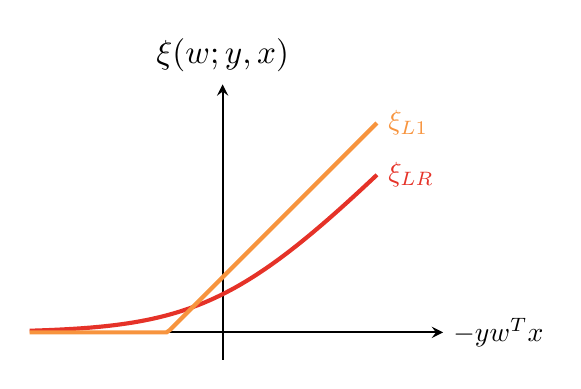
\begin{tikzpicture}[>=stealth, scale=0.7]
        % 定義與圖片相近的顏色
            \definecolor{customOrange}{RGB}{247, 148, 62} % 亮橘色
            \definecolor{customRed}{RGB}{229, 50, 40}    % 紅色

            % --- 繪製坐標軸 ---
            % X軸
            \draw[->, thick] (-3.5,0) -- (4,0) node[right] {$-y \bm{w}^T \bm{x}$};
            % Y軸
            \draw[->, thick] (0,-0.5) -- (0,4.5) node[above, scale=1.2] {$\xi(\bm{w}; y, \bm{x})$};

            % --- 繪製曲線 ---
            
            % 1. Logistic Regression (紅色曲線, LR)
            % 函數近似: log(1 + exp(x))
            \draw[customRed, line width=1.5pt, domain=-3.5:2.8, samples=100] 
                plot (\x, {ln(1+exp(\x))}) node[right] {$\xi_{\text{LR}}$};

            % 2. L1 / Hinge Loss (橘色曲線, L1)
            % 函數近似: max(0, x+1)
            % 為了視覺效果,我們用兩段線條畫出:一段平的,一段斜率為1的
            % 轉折點設在 x = -1
            \draw[customOrange, line width=1.5pt, domain=-3.5:2.8, samples=100] 
                plot (\x, {max(0, 1 + \x)}) node[right] {$\xi_{\text{L1}}$};


        \end{tikzpicture}
        \caption{Comparison of Logistic Loss and Hinge Loss}
    \end{figure}

    And logistic regression is very related to SVM, they look very similar in on the graph.
\end{note}

\subsection{Overfitting}

Minimizing the training error alone may not give a good model, as it may lead to overfitting. For classification, you can easily achieve 100\% training accuracy. But the model may not generalize well to unseen data.

In the following figure, model perfectly classifies all training data, but the perfermance on test data is not quite perfect.

\begin{figure}[H]
    \centering
    \includegraphics[width=0.7\textwidth]{Figures/Overfitting.png}
    \caption{Overfitting Example}
\end{figure}

If we just give up some training accuracy (might misclassify some training data), consider them to be the noise, we may get a better model that generalizes well to unseen data(margin 比較大)。

\begin{figure}[H]
    \centering
    \includegraphics[width=0.7\textwidth]{Figures/CorrectTraining.png}
    \caption{Regularization Example}
\end{figure}

\newpage

\subsection{Regularization}

Hence, we introduce regularization to our optimization problem, which helps to make the value of $\|\bm{w}\|$ less extreme. One idea of regularization is to make $\|\bm{w}\|$ close to zero. For example, we can add \[
    \frac{\bm{w}^\top \bm{w}}{2}\ (\text{which is } \| \bm{w} \|_2^2 \cdot \frac{1}{2}) \quad \text{ or } \quad \|\bm{w}\|_1 = \sum_{i=1}^{n} |w_i|
\]
\begin{note}
    加上 penalty term $\frac{\bm{w}^\top \bm{w}}{2}$ 會讓這一個 $\|\bm{w}\|$ 變得不容易很大。因為當 $\|\bm{w}\|$ 很大時,$\frac{\bm{w}^\top \bm{w}}{2}$ 也會迅速增加。$\min_{\bm{w}} f(\bm{w})$ 就會把這個雖然符合,但 margin 太小。
    假設點落在 margin 上,we get \[
        | \bm{w}^\top \bm{x} | = 1
    \]
    這樣我們可以得到兩條 margin lines 之間的距離是 
    \[
        \text{distance} = \frac{|C_1 - C_2|}{\sqrt{w_1^2 + w_2^2}} = \frac{2}{\|\bm{w}\|}
    \]
    當 $\|\bm{w}\|$ 越小,margin distance 就越大,代表這個 classifier 越 generalize
\end{note}

Therefore, the optimization problem becomes

\begin{definition}[General Form of Linear Classification]
    Let training data be \[
        \{y, \bm{x}_i\}, \ \bm{x}_i \in \mathbb{R}^n, \ y_i \in \{+1, -1\}, \quad \text{ for } i = 1, 2, \ldots, l
    \]
    where \(l\) is \# of training instances, $n$ is \# of features. The general form of linear classification optimization problem is \[
        \min_{\bm{w}} f(\bm{w}), \quad f(\bm{w}) = \frac{\bm{w}^\top \bm{w}}{2} + C \sum_{i=1}^{l} \xi(\bm{w}; \bm{x}_i, y_i)
    \]
\end{definition}

where \(C > 0\) is a hyperparameter that controls the trade-off between minimizing the training error and minimizing the model complexity (regularization term).

\section{Fully-connected Networks}

\subsection{Multi-class Classification}

\begin{definition}
    The training set of a fully-connected network is the same as linear classification. \[
        (\bm{y}^i, \bm{x}^i), \quad i = 1, 2, \ldots, l
    \]
    where \(\bm{y}^i \in \mathbb{R}^K\) is the label vector (one-hot encoding) and \(\bm{x}^i \in \mathbb{R}^n_1\) is the feature vector. 
\end{definition}


Due to the label is a vector now, we change \[
    \text{(label, instance)}: (\bm{y}_i, \bm{x}_i) \quad \to \quad \text{(label vector, instance)}: (\bm{y}^i, \bm{x}^i)
\]
where \(K\) is the number of classes and \(n_1\) is the number of features. If $x^i$ is in class $k$ then \[
    \bm{y}^i = [0, 0, \ldots, 1, \ldots, 0]^\top \in \mathbb{R}^K
\]

A neural network maps each input feature vector to one of the class labels by the connection nodes. Betewwn layers, there are weights matrix maps input to the next layer output.

\newpage

\subsection{Operation Between Layers}

\begin{figure}[H]
    \centering
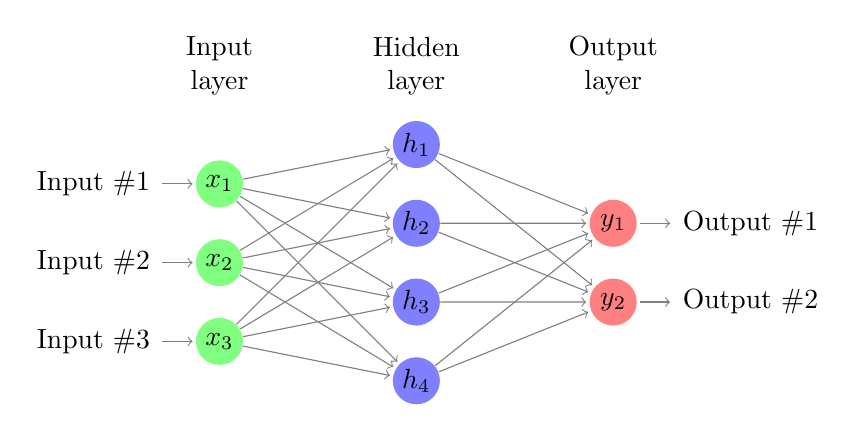
\begin{tikzpicture}[
    % 定義樣式
    shorten >=1pt,->,
    draw=black!50,
    node distance=2.5cm,
    every pin edge/.style={<-,shorten <=1pt},
    neuron/.style={circle,fill=black!25,minimum size=17pt,inner sep=0pt},
    input neuron/.style={neuron, fill=green!50},
    output neuron/.style={neuron, fill=red!50},
    hidden neuron/.style={neuron, fill=blue!50},
    annot/.style={text width=4em, text centered}
]

    % 設定各層的數量
    \def\inputNum{3}
    \def\hiddenNum{4}
    \def\outputNum{2}

    % --- 1. 繪製 Input Layer ---
    \foreach \name / \y in {1,...,\inputNum}
        \node[input neuron, pin=left:Input \#\y] (I-\name) at (0,-\y) {$x_{\y}$};

    % --- 2. 繪製 Hidden Layer ---
    % 這裡做了一個位移,讓它稍微置中一點 (視需求調整)
    \foreach \name / \y in {1,...,\hiddenNum}
        \path[yshift=0.5cm]
            node[hidden neuron] (H-\name) at (2.5cm,-\y) {$h_{\y}$};

    % --- 3. 繪製 Output Layer ---
    \foreach \name / \y in {1,...,\outputNum}
        \path[yshift=-0.5cm]
            node[output neuron, pin={[pin edge={->}]right:Output \#\y}] (O-\name) at (5cm,-\y) {$y_{\y}$};

    % --- 4. 連接線 (Edges) ---
    
    % 連接 Input -> Hidden
    \foreach \source in {1,...,\inputNum}
        \foreach \dest in {1,...,\hiddenNum}
            \path (I-\source) edge (H-\dest);

    % 連接 Hidden -> Output
    \foreach \source in {1,...,\hiddenNum}
        \foreach \dest in {1,...,\outputNum}
            \path (H-\source) edge (O-\dest);

    % --- 5. 加上標籤 (Labels) ---
    \node[annot,above of=H-1, node distance=1cm] (hl) {Hidden layer};
    \node[annot,left of=hl] {Input layer};
    \node[annot,right of=hl] {Output layer};

\end{tikzpicture}
\caption{A Simple Fully-connected Neural Network}
\end{figure}

The weight matrix $W^m$ at layer \(m\) is \[
    W^m = \begin{pmatrix}
        w_{11}^m & w_{12}^m & \cdots & w_{1 n_{m}}^m \\
        w_{21}^m & w_{22}^m & \cdots & w_{2 n_{m}}^m \\
        \vdots   & \vdots   & \ddots & \vdots       \\
        w_{n_{m+1} 1}^m & w_{n_{m+1} 2}^m & \cdots & w_{n_{m+1} n_{m}}^m
    \end{pmatrix}_{n_{m+1} \times n_{m}}
\]
where 
\begin{itemize}
    \item $n_m$ is the number of input features at layer \(m\).
    \item $n_{m+1}$ is the number of output features at layer \(m\).
    \item $w_{ij}^m$ is the weight connecting the \(j\)th node in layer \(m\) to the \(i\)th node in layer \(m+1\).
    \item $L$ is the total number of layers.
    \item $n_1$: number of features, $n_{L+1}$: number of classes.
\end{itemize}

Let $\bm{z}^m$ be the input of the \(m\)-th layer, $\bm{z}_1 = \bm{x}$ and $\bm{z}_{L+1} = \bm{y}$. From \(m\)-th layer to \((m+1)\)-th layer, the operation is \begin{align*}
    \bm{s}^m &= W^m \bm{z}^m \\
    \bm{z}_j^{m+1} &= \sigma(\bm{s}_j^m), \quad j = 1, 2, \ldots, n_{m+1}
\end{align*}

where 
\begin{itemize}
    \item $\sigma(\cdot)$ is the activation function.
\end{itemize}

Usually, we do a bias term $\bm{b}^m$ addition \[
    \begin{pmatrix}
        b_1^m \\
        b_2^m \\
        \vdots \\
        b_{n_{m+1}}^m
    \end{pmatrix}_{n_{m+1} \times 1}
\]
so that \[
    \bm{s}^m = W^m \bm{z}^m + \bm{b}    ^m
\]

\begin{note}[Actication Functions]
    Activation function $f$ is usually a scalar function \[
        f: \mathbb{R} \to \mathbb{R}
    \]
    for nonlinear transformation. 有些分類問題並非是 linear separable 的,所以需要這種 non-linear 來幫助分類,例如:
    \begin{itemize}
        \item Sigmoid: \(\sigma(x) = \frac{1}{1 + e^{-x}}\)
        \item Tanh: \(\tanh(x) = \frac{e^x - e^{-x}}{e^x + e^{-x}}\)
        \item ReLU: \(\text{ReLU}(x) = \max(0, x)\)
    \end{itemize}
    如果沒有 activation function,整個 network 就只是 linear transformation 的組合,等同於 single layer 的 linear model
    \[
        W^L W^{L-1} \cdots W^1 \bm{x} + \text{bias terms}
    \]
    如果做了 activation function,network 就沒辦法簡化成 single layer

\begin{figure}[H]
    \centering
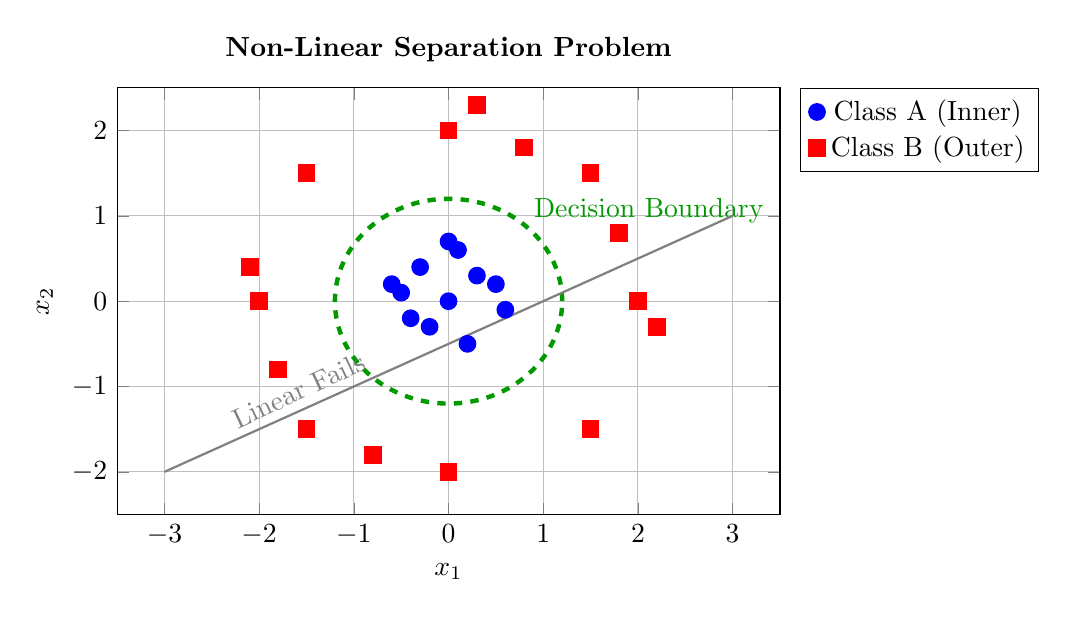
\begin{tikzpicture}
    \begin{axis}[
        title={\textbf{Non-Linear Separation Problem}},
        xlabel={$x_1$},
        ylabel={$x_2$},
        legend pos=outer north east,
        grid=major,
        width=10cm,
        height=7cm,
        xmin=-3.5, xmax=3.5,
        ymin=-2.5, ymax=2.5
    ]

    % Class 1 (Inner Circle - 藍色點)
    % 代表位於中心的一群資料
    \addplot[
        only marks,
        mark=*,
        color=blue,
        mark size=3pt
    ] coordinates {
        (0,0) (0.5,0.2) (-0.3,0.4) (0.2,-0.5) (-0.4,-0.2)
        (0.1,0.6) (-0.5,0.1) (0.3,0.3) (-0.2,-0.3)
        (0.6,-0.1) (-0.6,0.2) (0, 0.7)
    };
    \addlegendentry{Class A (Inner)}

    % Class 2 (Outer Ring - 紅色方塊)
    % 代表包圍在外圈的資料
    \addplot[
        only marks,
        mark=square*,
        color=red,
        mark size=3pt
    ] coordinates {
        (2,0) (-2,0) (0,2) (0,-2)
        (1.5,1.5) (-1.5,1.5) (1.5,-1.5) (-1.5,-1.5)
        (1.8,0.8) (-1.8,-0.8) (0.8,1.8) (-0.8,-1.8)
        (2.2, -0.3) (-2.1, 0.4) (0.3, 2.3)
    };
    \addlegendentry{Class B (Outer)}

    \draw[green!60!black, ultra thick, dashed] (axis cs:0,0) circle [radius=1.2];
    \node[green!60!black, anchor=south west] at (axis cs: 0.8, 0.8) {Decision Boundary};

    \addplot[domain=-3:3, samples=2, color=gray, thick] {0.5*x - 0.5};
    \node[gray, rotate=25, anchor=south] at (axis cs: -1.5, -1.25) {Linear Fails};

    \end{axis}
\end{tikzpicture}
\caption{Non-Linear Separation Problem}
\end{figure}

\end{note}

To simplify the notation, we denote all the variables as a vector \(\theta\) \[
    \theta = \begin{pmatrix}
        \text{vec}(W^1) \\
        \bm{b}^1 \\
        \vdots \\
        \text{vec}(W^L) \\
        \bm{b}^L
    \end{pmatrix} \in \mathbb{R}^n
\]
where $n$ is total $\#$ parameters in the network $ = (n_1 +1) n_2 + \cdots (n_L + 1) n_{L+1}$. And the operator $$\text{vec}(\cdot)$$ stacks the columns of a matrix into a vector.

\newpage

The optimization problem for training a fully-connected network should be write in 
\begin{definition}[Optimization Problem for Fully-connected Network]
    For $\theta$ is the parameter vector, the optimization problem for training a fully-connected network is
    \[
        \min_{\theta} f(\theta), \quad f(\theta) = \frac{1}{2} \theta^\top \theta + C \sum_{i=1}^{l} \xi(z^{L+1, i}(\theta); \bm{y}^i, \bm{x}^i)
    \]
\end{definition}

where
\begin{itemize}
    \item \(C\): regularization hyperparameter.
    \item \(z^{L+1}(\theta) \in \mathbb{R}^{n_{L+1}}\): last layer output (predicted label vector) of the feature $\bm{x}$
    \item \(\xi(z^{L+1}(\theta); \bm{y}, \bm{x})\): loss function: for instance \[
        \xi(z^{L+1}(\theta); \bm{y}, \bm{x}) = \| z^{L+1}(\theta) - \bm{y} \|^2
    \]
\end{itemize}

This is similar to the linear classification problem, but now the model is more complex. Futher, the optimization problem is non-convex due to the non-linear activation functions and multiple layers. 
\begin{remark}
    In the real world, deep learning models often have not single instance, so in the process of training, it is actually for $i = 1, \ldots, l$
    \begin{align*}
        \bm{s}^{m, i} &= W^m \bm{z}^{m, i} + \bm{b}^m \\
        \bm{z}_j^{m+1, i} &= \sigma(\bm{s}_j^{m, i}), \quad j = 1, 2, \ldots, n_{m+1}
    \end{align*}
\end{remark}

